\documentclass[12pt,titlepage,dvipdfmx]{jarticle}

%お好みに合わせて変えてください
\usepackage[top=30truemm,bottom=30truemm,left=25truemm,right=25truemm]{geometry}
\usepackage{hyperref}
\usepackage{amsmath,amssymb}
\usepackage[utf8]{inputenc}
\usepackage{physics}
\usepackage{color}
\usepackage{url}
\usepackage{here}
\usepackage{ascmac}
\usepackage[dvipdfmx]{graphicx}
\usepackage{siunitx}


\hypersetup{
    colorlinks=true,
    linkcolor=blue,
    filecolor=magenta,      
    urlcolor=cyan,
    pdftitle={Sharelatex Example},
    %bookmarks=true,
    pdfpagemode=FullScreen,
}

\title{カゴメ格子上の$J_1 - J_2$古典反強磁性$XY$模型の有限温度相図(仮)}
\author{埼玉大学大学院理工学研究科 博士前期課程\\物理機能系専攻 物理学コース\\20MP104 柿澤文哉 }

\begin{document}

\maketitle

\newpage

\begin{abstract}
[ここにアブストラクトを書く。
本研究では典型的な幾何学的フラストレート磁性体であるカゴメ格子上の最近接古典反強磁性$XY$模型に次近接相互作用$J_2$を導入した模型(図xx)に対して、
大規模なモンテカルロ計算を行い、有限温度相図($J_2-T$相図)を作成し、各相における秩序構造や各相の関係を解明することを目的に行われた。
以下の各章で、
\begin{itemize}
   \item 古典スピン模型
   \item 相転移現象
   \item 幾何学的フラストレート磁性体
   \item モンテカルロ法による解析手法
\end{itemize}
について説明する。]


\end{abstract}

\tableofcontents

\newpage

\newpage 

\section{イントロダクション}
\subsection{{古典スピン模型}}
磁性は原子・電子が持つスピン自由度がマクロな数存在することによって発現する。
現代の磁性研究の主流は、ミクロな構成要素であるスピンとスピン間の相互作用から出発し、磁性というマクロな性質を説明することである。
物質中のスピン間の相互作用を記述するのが(局在)古典スピン模型である。
$N$体のスピン系を仮定すると、最大$N$体の相互作用が考えられるが、二体の交換相互作用のみを考えれば、
強磁性など典型的な磁性を説明できる。ハミルトニアンは以下で与えられる。
\begin{align}
   H = \sum_{(ij)} J_{ij} \vec{S}_i\cdot \vec{S}_j.
\end{align}
$\vec{S}_i$は格子点$i$上で定義される単位ベクトルを表し、$J_{ij}$は交換相互作用を表す。
$(ij)$は互いに交換相互作用を及ぼすスピンの組を表す。
理論上、$\vec{S}$の次元に制限はないが、磁性研究では三次元までが対象となることが多く、次元に応じて
\begin{itemize}
   \item $\vec{S}=S^z$の場合、イジング(Ising)スピン
   \item $\vec{S}=(S^x,S^y)$の場合、$XY$スピン
   \item $\vec{S}=((S^x,S^y,S^z)$の場合、ハイゼンベルグ(Heisenberg)スピン
\end{itemize}
と呼ばれる。
%スピンがイジング/$XY$/ハイゼンベルグスピンであるとき、古典スピン模型もイジング/$XY$/ハイゼンベルグ模型と呼ばれることがある。

強磁性と反強磁性は交換相互作用のみの模型によって強磁性と反強磁性を説明できる。
説明のために隣り合う格子点(最近接格子点)上のスピン間のみに交換相互作用が働くことを仮定する。
\begin{align}
   H_{\mathrm{NN}} = \sum_{\ev{ij}} J_{ij} \vec{S}_i\cdot \vec{S}_j. 
\end{align}
$J_{ij}<0\ (\forall{ij})$のとき、$\vec{S}_i\cdot\vec{S}_j=1\ (\forall{ij})$を満たす状態が最低エネルギーとなるが、
これはすべてのスピンが同方向に揃った強磁性状態である。
一方で、$J_{ij}>0\ (\forall{ij})$のとき、$\vec{S}_i\cdot\vec{S}_j=-1\ (\forall{ij})$の状態が最低エネルギーとなるが、
これは隣り合うすべてのスピンが互いに逆方向を向いた反強磁性状態である。
これを以て$J_{ij}<0$を強磁性的、$J_{ij}>0$を反強磁性的(交換相互作用)と呼ぶ。

上の議論から$J_{ij}=0\ (\forall{ij})$を境に系の最低エネルギー状態が強磁性/反強磁性状態から反強磁性/強磁性状態へ定性的に変化する。
(厳密には$J_{ij}=0$の最低エネルギー状態は任意のスピン配置なので、$J_{ij}=0$は含まない。)
また、これまでの議論では暗に絶対零度($T=0$)を仮定していたが、高温極限$(J/T<<1)$ではスピンが何ら秩序を示さない常磁性状態が支配的となり、
系は常磁性を示す。したがって、絶対零度から温度を上昇させていったとき、ある温度を境に系の磁性が(反)強磁性から常磁性へ定性的に変化することが想像される。
このように何らかのパラメータを連続的に変化させたとき、ある値を境に系の性質が定性的かつ不連続に変化する現象を相転移現象という。

%次節では相転移現象一般について述べた後、特に磁性体に関連する過去の相転移研究の結果を紹介する。

\newpage

\subsection{相転移現象}
相転移現象(以降、単に相転移)は、何らかのパラメータを連続的に変化させたとき、ある値を境に系の性質が定性的かつ不連続に変化する現象を指す。
より詳細に述べると、相転移前後の同一の性質を示すパラメータ領域を相といい、パラメータ変化に伴い、
相間を移ることによって、系の性質が定性的かつ不連続に変化する。
現代の相転移研究では、それぞれの相は相の秩序構造を反映した物理量である秩序変数によって特徴づけられ、相転移は秩序変数の不連続変化によって記述されることが多い。
また、相転移は次数によっても特徴づけられる。$n$次相転移の定義は自由エネルギー$F$の$n$階微分$\pdv*[n]{F}{X}$が転移点$X=X_{\mathrm{c}}$で発散することである。


相転移の最も身近な例として水における相転移が挙げられる。
水の場合はパラメータとして圧力$P$と温度$T$を使うことが多く、$P-T$平面($P-T$相図)に固相・液相・気相が存在する。
大気圧下では$0\si{\degreeCelsius}$において固体ー液体相転移、$100\si{\degreeCelsius}$において液体ー気体相転移を示す。
(摂氏温度における$0\si{\degreeCelsius}$と$100\si{\degreeCelsius}$の定義)。
ここでの秩序変数は密度であり、$0\si{\degreeCelsius}$と$100\si{\degreeCelsius}$で不連続に変化することが知られている。
固体ー液体相転移と液体ー気体相転移はともに一次相転移である。

本題である磁性体に関する相転移について説明する。
磁性体に関する相転移における最も重要な定理の一つとして、マーミン・ワグナーの定理がある。
この定理は以下を主張している。[ステートメントが不正確かもしれない。後で修正する。]
\begin{center}
   二次元以下の格子では、有限温度で連続対称性の自発的破れを伴う相転移は存在しない。
\end{center}
以下、対称性の自発的破れについて説明する。まず、離散対称性の場合を議論する。
簡単のため、最近接相互作用のみの二次元正方格子上のイジング模型を考える。強磁性的な相互作用を仮定する。
この模型は厳密解が存在し、有限温度$T=T_{\mathrm{c}}$で二次相転移を示すことが分かっている。
$T<T_{\mathrm{c}}$では強磁性状態が支配的となり、$T=0$では全てのスピンが$S_i^z=1$あるいは$S_i^z=-1$に揃っている。
これら二つの状態はエネルギー的に縮退しているため、エネルギーの損得はないが、必ずどちらかが選ばれる。
この状況を全スピンに対する反転対称性が自発的に破れている、という。
同じように、$XY$/ハイゼンベルグ模型などの連続対称性を示す模型において基底状態から唯一つ状態が選ばれることを
連続対称性の自発的破れという。マーミン・ワグナーの定理はそのような連続対称性の破れを伴う有限温度での相転移が、
二次元格子系では存在しないことを主張している。

%では、マーミン・ワグナーの定理があるため、二次元以下の格子上の$XY$/ハイゼンベルグ模型について、もはや
%興味深い問題は残っていないのだろうか。
%答えは否で、本研究で扱う幾何学的フラストレート磁性体という複数の相互作用が拮抗するスピン模型は
%\begin{itemize}
%   \item BKT転移[発見者3名の名前を忘れた。後で調べておく。]
%   \item (幾何学的)フラストレート磁性体
%   \item カイラリティなどの、離散対称性を示す新規秩序
%\end{itemize}
%が挙げられる。本節ではBKTについてのみ説明し、残りの二つは次節以降で説明する。

\newpage

\subsection{幾何学的フラストレート磁性体}
相互作用によるエネルギー利得を局所的に最大化する条件が系全体で同時に満足できない状況を、フラストレーションがあるという。
特に、格子の幾何学的特徴によるフラストレーションを幾何学的フラストレーション、磁性体を幾何学的フラストレート磁性体という。
最も簡単な幾何学的フラストレート磁性体は三角形上の反強磁性イジング模型である。この模型を用いて(幾何学的)フラストレーションを説明する。

\begin{figure}[tbh]
   \centering
   \includegraphics[width=5cm]{figure/triangle_Ising_AFM.pdf}
   \caption{三角形上の反強磁性イジング模型}
\end{figure}
   
まず、相互作用を得するよう、上サイトにアップスピン、左下サイトにダウンスピンを配置する。右下のサイトにスピンを配置する。
上サイトのスピンとの相互作用利得を最大化するためにはダウンスピンを配置すればよいが、このとき左下サイトのスピンとは最大化できない。
アップスピンを配置した場合でも事情は同様である。
したがって、三つのスピンが互いに逆向きであるという局所的エネルギー利得最大化条件を系全体で同時に満足できない。
%この状況を指して、系にフラストレーションがあるといい、さらにフラストレーションが三角形という幾何学的特徴に由来するため、この系には幾何学的フラストレーションがある、という。

いくつかの幾何学的フラストレート磁性体は、マクロ系において基底状態の縮退数が格子点数に対して指数関数的に増加するという顕著な性質を示す。
これを基底状態の巨視的縮退という。巨視的縮退数は格子やスピンの種類で変化する。
本研究の主題であるカゴメ格子上の古典反強磁性$XY$模型は次節以降に譲り、本章では三角格子とカゴメ格子上の古典反強磁性イジング模型について過去の結果を整理する。

%\subsection{基底状態の巨視的縮退}
%フラストレート系の最大の特徴は、三角形を結合したマクロな格子系において、基底状態の縮退数がスピン数に対して指数関数的に増加することである。
%このような縮退を巨視的縮退という。
%本節では、まず非自明な縮退について述べ、二つの三角形を結合したフラストレート系において三角形模型よりも基底状態の縮退数が増加することを見て、
%最後にマクロなフラストレート系の代表例である三角格子とカゴメ格子の巨視的縮退について過去の結果を紹介する。
%
%非自明な縮退を考える前に、まず自明な縮退として、正方格子上の反強磁性イジング模型における基底状態の縮退を考える。
%この模型の基底状態はアップスピンとダウンスピンが交互に並ぶ状態であるが、この状態は全てのスピンが反転した状態とだけ縮退している。
%この縮退はハミルトニアンの対称性から明らかであるため、自明な縮退である。
%非自明な縮退として、やはり三角形上の反強磁性イジング模型における基底状態の縮退を考える。
%この模型の基底状態は異なる三つの状態にそれぞれ自明な二重縮退があり、六重縮退している。
%三つの状態は全スピン反転によって互いに行き来できないため、ハミルトニアンの対称性に由来しない非自明な縮退となっている。
%
%自明な縮退における縮退数は高々ハミルトニアンの対称性程度$\mathcal{O}(1)$であるため、マクロな格子系における巨視的縮退をもたらすのは非自明な縮退である。
%ここから、辺共有結合三角形上の反強磁性イジング模型(辺共有模型、図2)と頂点共有結合三角形上の反強磁性イジング模型(頂点共有模型、図3)を用いて、
%非自明な縮退がある場合、どちらの模型の基底状態においても縮退数が三角形模型より増加すること、辺共有模型よりも頂点共有模型の方が縮退数が多いことを示す。
%
%\begin{figure}[tbh]
% \begin{minipage}{0.5\hsize}
%  \begin{center}
%   \includegraphics[width=50mm]{figure/edge_shared_triangle.pdf}
%  \end{center}
%  \caption{辺共有三角形上のイジング模型}
%  \label{fig:one}
% \end{minipage}
% \begin{minipage}{0.5\hsize}
%  \begin{center}
%   \includegraphics[width=55mm]{figure/top_shared_triangle.pdf}
%  \end{center}
%  \caption{頂点共有三角形上のイジング模型}
%  \label{fig:two}
% \end{minipage}
%\end{figure}
%
%まず辺共有模型の基底状態を考える。図2の上向き三角形だけを見れば三角形模型と同じであるから、図1と同じようにスピンを配置すればよい。
%右上のサイトにはどちらのスピンを配置すればよいか。右下サイトにアップスピンが入った場合はダウンスピンを配置すればよい。
%問題はダウンスピンが入った場合で、このときは右上のサイトがフラストレートしてしまう。したがって辺共有模型は三角形模型より基底状態における縮退数が多い。
%次に頂点共有模型を考える。先と同様に図3の左の三角形に図1と同じようにスピンを配置しよう。残った右の三角形の上下サイトにスピンを配置する。
%共有サイトとエネルギー利得を最大化するように上サイトにスピンを配置すると、下サイトは三角形模型と同じ理由でフラストレートする。
%はじめに下サイトにスピンを配置しても事情は同じである。したがって頂点共有模型も三角形模型より基底状態における縮退数が多い。
%また、辺共有模型と頂点共有模型を比べると頂点共有模型の方が縮退数が多い。
%これは共有しているサイトが少なく、フラストレートしているサイトのうち一つのスピンを決めても、これによってスピンが決まるサイトが少ないためである。
%
%最後に、マクロなフラストレート系の代表例である三角格子上の反強磁性イジング模型(三角格子模型、図xx)と
%カゴメ格子上の反強磁性イジング模型(カゴメ模型、図xx)における基底状態の巨視的縮退について過去の結果を紹介する。
%
%ここまで見てきたように、マクロなフラストレート系において、基底状態が巨視的に縮退し、絶対零度まで相転移が抑制される場合がある。
%これを踏まえて、初期のフラストレート系研究では縮退数や低温下のスピン相関の空間構造などが研究されてきたが、
%近年になって、巨視的縮退が外部磁場や異方性などの摂動によって敏感に解消され、有限温度において相転移を示すことが分かってきた。
%
%本研究では摂動としてより一般的かつ現実的な次近接相互作用$J_2$を導入し、有限温度での振る舞いを調べた。研究に用いた模型、先行研究、動機の詳細は次章で述べる。
%
\newpage

%\section{本研究の動機・目的}
%%[話の流れは、動機・目的→先行研究→動機・目的、じゃないとおかしいか。]
%本研究の目的はカゴメ格子上の$J_1-J_2$古典反強磁性$XY$模型(図xxx)を対象に、幾何学的フラストレート磁性体を舞台とした次近接相互作用$J_2$と
%温度$T$の協奏効果を明らかにすることである。具体的には次近接相互作用$J_2$や温度$T$の効果によって、どのような秩序相が現れるか、
%また、相転移にはどのような特徴があるかなどの問題を解決することである。
%\begin{center}
%   put image of $J_1-J_2$ model
%\end{center}
%このような問題を議論するためには、$J_2-T$相図
%
%%したがって、相図の作成において、ある領域にどのような秩序相が存在するか予想し、それぞれの秩序に対応した秩序変数を構成することが重要となる。
%
%

\newpage

%\section{先行研究}
\section{カゴメ格子上の$J_1-J_2$古典反強磁性$XY$模型}
\subsection{$J_2=0$}
ハミルトニアンは
\begin{align}
   H_{\mathrm{NN}} = \sum_{\ev{ij}}J_{ij}\vec{S}_i\cdot\vec{S}_j
\end{align}
$\ev{ij}$は最近接格子点の組を表す。$J_{ij}=1\ (\forall{ij})$とする。
\subsubsection{$T=0$}
ハミルトニアンを副格子ごとの和で書き直す。
\begin{align}
   H_{\mathrm{NN}} = \sum_{\mathrm{sublattice}} (\vec{S}_1+\vec{S}_2+\vec{S}_3)^2 + \mathrm{const.}
\end{align}
添字は副格子内の格子点を表す。よって、基底状態は各副格子内で以下の条件を満たす。
\begin{align}
   \vec{S}_1+\vec{S}_2+\vec{S}_3 = 0
\end{align}
この条件を満たす副格子内のスピン配置として、以下の$120^\circ$構造がある。
\begin{figure}[tbh]
   \centering
   \includegraphics[width=10cm]{figure/120degs_structures.pdf}
   \caption{カイラリティ符号が異なる二つの$120^\circ$構造}
\end{figure}

$120^\circ$構造はカイラリティ自由度によって特徴づけれられる。
カイラリティは副格子ごとに
\begin{align}
   \kappa \equiv \frac{2}{3\sqrt{3}}(\vec S_1 \times \vec S_2 + \vec S_2 \times \vec S_3 + \vec S_3 \times \vec S_1)
\end{align}
で定義される。
全系の基底状態は各副格子に$120^\circ$構造を配置して得られる。
縮退数$N_{\mathrm{GS}}$はBaxterによって三色問題の解であることが指摘された。
現在では、格子点数を$N$として
\begin{align}
   N_{\mathrm{GS}} = 1.13471^{N}
\end{align}
であり、巨視的縮退を示すことが知られている。

[田畑氏のレビューによると、Baxterの数値は間違っていて、後年修正されたという。]
%・三角格子状の反強磁性$XY$模型の基底状態は巨視的縮退を示さない。


\subsubsection{T≠0}
\begin{itemize}
   \item 有限温度での八極子準長距離秩序のBKT転移が存在する
   \item 八極子相は磁気的準長距離秩序が存在しつつ、カイラリティ長距離秩序が存在しない相である。
   \item 
\end{itemize}
\newpage

\subsection{J2≠0}

\subsubsection{T=0}

\begin{figure}[tbh]
   \begin{minipage}{0.5\hsize}
    \begin{center}
     \includegraphics[width=6cm]{figure/q0.pdf}
    \end{center}
    \caption{$q=0$構造}
    \label{fig:one}
   \end{minipage}
   \begin{minipage}{0.5\hsize}
    \begin{center}
     \includegraphics[width=5cm]{figure/sqrt3.pdf}
    \end{center}
    \caption{$\sqrt{3}\times\sqrt{3}$構造}
    \label{fig:two}
   \end{minipage}
  \end{figure}
\begin{itemize}
   \item 基底状態の巨視的縮退が$J_2$によって解消され、$\sqrt{3}\times\sqrt{3}(J_2/J_1>0)$構造、$q=0(J2/J1<0)$構造が基底状態となる。
   \item $\sqrt{3}\times\sqrt{3}$構造は反強磁性的カイラリティ、$q=0(J_2/J_1<0)$構造は強磁性的カイラリティを示す。
\end{itemize}


\subsubsection{T≠0}
\begin{figure}[tbh]
   \centering
   \includegraphics[width=15cm]{figure/schematic_phase_diagram.pdf}
   \caption{現象論的$J_2-T$相図}
\end{figure}

\begin{itemize}
   \item S.E.Korshunovによる現象論によって得られた概念的な$J_2-T$相図を示す。
   \item 磁気的準長距離秩序($\sqrt{3}\times\sqrt{3}$秩序と$q=0$秩序)は有限温度でBKT転移を示す。
   \item カイラリティ長距離秩序も磁気的準長距離秩序と同時に転移する。
   \item $J_2=0$での八極子転移が$J_2\neq0$にも残り、$\sqrt{3}\times\sqrt{3}$相と$q=0$相との中間相となる。
   \item 八極子相の転移温度は$J_2$に依存せず一定である。
   \item 相図の原点近傍に$\sqrt{3}\times\sqrt{3}$相が$J_2/J_1<0$側に張り出す構造がある。
\end{itemize}
\newpage

\section{本研究の動機・目的}
%[動機と目的は違う言葉か。ニュアンスが微妙。]
先行研究を踏まえ、本研究で取り組むべき問題を再定義する。
その前に、先行研究で分かった点と分からなかった点をそれぞれ整理しておこう。

分かった点。$J2_T$相図を見れば分かることは書かない。
\begin{itemize}
   \item $J_2=0$の基底状態は巨視的縮退を示す。
   \item 警告。書き方に迷うので後回しにする。忘れるなかれ。
   \item 八極子-常磁性転移のBKT温度$T_{\mathrm{BKT}}$は$J_2$によらず一定。
\end{itemize}

分からなかった点
\begin{itemize}
   \item 転移温度$T_c$の数値
   \item 相転移の特徴
   \item $J_2<0(\abs{J_2}\ll1)$のでっぱり。
   \item 相転移の機構
\end{itemize}

\newpage


\newpage

\section{計算手法}

数値計算にはモンテカルロ法を用いた。モンテカルロ法は乱数を用いた数値計算手法の総称である。
本章では、本研究で用いた平衡法と非平衡緩和法について説明する。

\subsection{平衡法}
\subsubsection{計算する物理量}

平衡法では物理量$Q$の熱力学平均
\begin{align}
   \ev{Q} \equiv \frac{\sum_{S\in\Omega}e^{-\beta H(S)}Q(S)}{\sum_{S\in\Omega}e^{-\beta H(S)}}
\end{align}
を計算できる。ここで、$\Omega$は状態空間、$S$は状態、$H$は系のハミルトニアン、$\beta=1/k_{\mathrm{B}}T$は逆温度である。
以降、$k_{\mathrm{B}}=1$とする。本研究で計算する物理量とそれぞれの定義を以下に列挙する。(順不同)

比熱
\begin{align}
   C \equiv \frac{\ev{E^2}-\ev{E}^2}{N_{\mathrm{site}}T^2}
\end{align}
$N_{\mathrm{site}}$は格子点の総数を表す。

磁気秩序変数
\begin{eqnarray}
   m^2_{\mathrm{\sqrt3\times\sqrt3}} &=& 
   \frac{1}{3N^2_{\mathrm{triangle}}}\sum_{l}\left[\sum_{i} \vec S_l^i \exp\left( \frac{2\pi\mathrm{i}}{3}(x_l^i+y_l^i)\right)\right]^2\\
   m^2_{q=0}                         &=& 
   \frac{1}{3N^2_{\mathrm{triangle}}}\sum_{l}\left(\sum_{i} \vec S_l^i \right)^2
\end{eqnarray}
添字$l$は副格子内の格子点番号を表す。

八極子秩序変数
\begin{align}
   m^2_{\mathrm{octupole}} \equiv 
\frac{1}{N_{\mathrm{site}}^2}\left[ \left(\sum_i \cos 3\theta_i \right)^2+\left(\sum_i\sin 3\theta_i\right)^2\right]
\end{align}
$\theta_i$は$i$番目のスピンについて$x$軸から測った角度を表す。

(反)強磁性的カイラリティ秩序変数
\begin{eqnarray}
   \kappa_{\mathrm{AFM}}^2 &=& 
   \left[ \frac{1}{N_{\Delta}}\sum_{\mathrm{all}\Delta}\kappa{\Delta} - \frac{1}{N_{\nabla}}\sum_{\mathrm{all}\nabla}\kappa_{\nabla}\right]^2\\
   \kappa_{\mathrm{FM}}^2  &=& 
   \left[ \frac{1}{N_{\Delta}}\sum_{\mathrm{all}\Delta}\kappa{\Delta} + \frac{1}{N_{\nabla}}\sum_{\mathrm{all}\nabla}\kappa_{\nabla}\right]^2
\end{eqnarray}
$\kappa_{\Delta,\nabla}$は前述したカイラリティで、計算する副格子(上向三角形$\Delta$と下向三角形$\nabla$)を明記した量である。
すなわち
\begin{align}
   \kappa_{\Delta,\nabla} = \frac{2}{3\sqrt{3}}(\vec S_1 \times \vec S_2 + \vec S_2 \times \vec S_3 + \vec S_3 \times \vec S_1)_{\Delta,\nabla}.
\end{align}
$N_{\Delta},N_{\nabla}$はそれぞれ上向三角形と下向三角形の数を表す($N_{\mathrm{triangle}}=N_{\Delta}+N_{\nabla}$)。

\subsubsection{シングルスピンフッリプアップデート}
本研究で使用したシングルスピンフリップアップデートを以下にまとめた。

\begin{itembox}[1]{シングルスピンフリップアップデート}
   \begin{enumerate}
       \item 適当な初期状態$\vec{C}_0=(\vec{S}_1,\vec{S}_2,\cdots,\vec{S}_{N_{\mathrm{spin}}})$を用意する。
       \item $\vec{C}_0$のエネルギー$E$を計算する。
       \item $\vec{S}_1$を選ぶ。
       \item $\vec{S}_1$と相互作用するスピンから有効磁場$\vec{h}_{\mathrm{eff}} = \sum _{(1,j)}J_{1j}\vec{S}_j$を計算する。
       \item 新しいベクトル$\vec{S}'_1$を提案する。
       \item 提案前後のエネルギー差$\Delta E = (\vec{S'}_1 - \vec{S}_1) \cdot \vec{h}_{\mathrm{eff}}$を計算する。
       \item 0以上1未満の乱数$r$を発生させ、$P = \exp(-\beta \Delta E)$よりも小さければベクトルを更新する。そうでなければ元のベクトルに「更新」する。
       \item 更新前後のエネルギー差$\Delta E$を$E$に加える。
       \item $\vec{h}_{\mathrm{eff}}$まわりに$\vec{S}_1$を$\pi$だけ回転させる。(オーバーリラクゼーション)
       \item 次のスピンに移り、$4\sim9$を繰り返す。
   \end{enumerate}
\end{itembox}

メモ
・一様ランダムフリップとガウシアンムーブ・物理量の計算

\newpage

\subsubsection{レプリカ交換法}

本研究で使用したレプリカ交換法のアルゴリズムを以下にまとめた。
\begin{itembox}[2]{レプリカ交換法}
\begin{enumerate}
    \item $\vec{\beta}$を用意し,それぞれのレプリカの初期状態を適当に決める。
    %\item 全てのレプリカに対してシングルスピンフリップアップデートを一斉かつ適当な回数行う。
    \item $\vec{\beta}$の一つ目に対応するレプリカを選ぶ。
    \item 現在のレプリカと右隣のレプリカの状態から$\Delta = (\beta_n - \beta_{n+1})\left(\mathcal{H}(S) - \mathcal{H}(S')\right)$を計算する。
    \item 0以上1未満の乱数$r$を発生させ、$r$が$\exp(-\Delta)$よりも小さければレプリカを交換する。
    \item 右隣のレプリカに移り4に戻る。右隣にレプリカがない場合6へ進む。
    \item 2に戻る。
\end{enumerate}
\end{itembox}

\subsubsection{ループアップデート}

\begin{figure}[tbh]
   \centering
   \includegraphics[width=10cm]{figure/loop_update.pdf}
   \caption{ループアップデートの概念図}
\end{figure}

\newpage

\subsection{非平衡緩和法}

\subsubsection{計算する物理量}
非平衡緩和法では以下で定義される秩序変数$O$の時間相関関数$G_O(t)$を計算する。
\begin{align}
   G_{O}(t) \equiv O(t) \cdot O(0).
\end{align}
時刻$t$は1MC stepを単位に測る。
1MC stepはすべてのスピンに対して一度シングススピンフリップアップデートをかけることと定義する。
$O(t)$は時刻$t$における秩序変数$O$の値を表す。
非平衡緩和法は$G_O(t)$の時間変化(緩和過程)から転移温度$T_{\mathrm{c}}$を推定する手法である。
%熱力学平均$\ev{O}$を計算しない、すなわち平衡分布への収束を必要としないため、平衡法に比べて大きなサイズの系を扱うことができる。

\subsubsection{非平衡緩和法の一般論}

$T>T_{\mathrm{BKT}}$では$G(t)$は指数関数的に減衰すると期待される。(空間相関関数からの類推)
\begin{align}
   G(t) =  a \ \mathrm e^{-t/\tau}.
\end{align}
$\tau$を緩和時間という。両辺の対数を取ると
\begin{align}
   \ln{G(t)} = \ln{a}-\frac{1}{\tau}t.
\end{align}
$\ln{G(t)}$から$\tau$を推定する。
$\tau$の温度依存性は転移温度近傍$T\sim T_{\mathrm{BKT}}$で
\begin{align}
   \tau = b \ \exp [c/(T-T_{\mathrm{BKT}})^{1/2}].
\end{align}
同じく両辺の対数を取って
\begin{align}
   \ln{\tau} = \ln{b} + \frac{c}{\sqrt{T-T_{\mathrm{BKT}}}}.
\end{align}
$\ln{\tau}$から$T_{\mathrm{BKT}}$を推定する。

カイラリティ転移の場合、転移温度近傍での$\tau$の温度依存性のみBKT転移と異なる。
\begin{align}
   \tau = b \ (T-T_{\mathrm{c}})^{-z\nu}.
\end{align}

本研究ではスケーリング則を利用し複数温度の$G(\tau)$から$\tau$を一度に推定する。

\newpage

\subsubsection{スケーリング則を利用した緩和時間の推定}

$T>T_{\mathrm{BKT}}$において、各温度における$G(t)$は以下のスケーリング則に従うと期待される。
\begin{align}
   g(t/\tau) = \tau_{\mathrm{exact}}^{\lambda_{\mathrm{BKT}}}G(t).
\end{align}
$\tau_{\mathrm{exact}}$は各温度で定義された緩和時間、$\lambda_{\mathrm{BKT}}$は$G(t)$の動的臨界指数を表す。
%$\lambda_{\mathrm{BKT}}$は時間と温度に依存しないと仮定する[動的臨界指数だとすると、by definiton?]
式(xx)の主張は、$T>T_{\mathrm{BKT}}$において、各温度で得られた$G(t)$とその温度における$\tau_{\mathrm{exact}}$を用いて計算した
$\tau_{\mathrm{exact}}^{\lambda_{\mathrm{BKT}}}G(t)$はすべての温度で一致する、である。
したがって、$\tau^{\lambda_{\mathrm{BKT}}}G(t)$が一致するように$\tau$を変化させていけば、最終的な結果は$\tau\sim\tau_{\mathrm{exact}}$となることが期待される。

具体的なアルゴリズムを以下にまとめる。
\begin{itembox}[1]{スケーリング則を利用した緩和時間$\tau$の推定アルゴリズム}
   \begin{enumerate}
       \item 
       \item 
       \item 
       \item 
   \end{enumerate}
\end{itembox}

[$\lambda$の扱いについて説明する。・$\lambda$も変分パラメータに含めたこと・その理由(動的臨界指数の値を知らない)・動的臨界指数の普遍性からおそらく時間/温度依存性がないと期待されること]
\newpage

\section{結果}
\subsection{$J2-T$相図}

\begin{figure}[tbh]
   \centering
   \includegraphics[width=15cm]{figure/phase_diagram.pdf}
   \caption{$J_2-T$相図}
\end{figure}

\subsection{比熱}

\begin{figure}[tbh]
   \centering
   \includegraphics[width=15cm]{figure/specific_heat.pdf}
   \caption{比熱の温度とサイズ依存性}
\end{figure}

\begin{figure}[tbh]
   \centering
   \includegraphics[width=15cm]{figure/cpeak_scaling.pdf}
   \caption{比熱ピークのスケーリング}
\end{figure}

\subsection{エネルギーヒストグラム}

\begin{figure}[tbh]
   \centering
   \includegraphics[width=15cm]{figure/egap_j2.pdf}
   \caption{エネルギーギャップの$J_2$依存性}
\end{figure}

\begin{figure}[tbh]
   \centering
   \includegraphics[width=15cm]{figure/energy_histogram.pdf}
   \caption{エネルギーヒストグラム[FK:字が読めない。gnuplotの設定レベルの問題ではない。]}
\end{figure}

\subsection{秩序変数}

\begin{figure}[tbh]
   \centering
   \includegraphics[width=15cm]{figure/order_params_q0.pdf}
   \caption{強磁性的カイラリティ秩序変数と$q=0$磁気秩序変数の温度依存性}
\end{figure}

\begin{figure}[tbh]
   \centering
   \includegraphics[width=15cm]{figure/order_params_sqrt3.pdf}
   \caption{反強磁性的カイラリティ秩序変数と$\sqrt{3}\times\sqrt{3}$磁気秩序変数の温度依存性}
\end{figure}

\begin{figure}[tbh]
   \centering
   \includegraphics[width=12cm]{figure/octupole_order_params.pdf}
   \caption{八極子秩序変数の温度依存性}
\end{figure}

\subsection{各秩序変数の緩和過程と緩和時間}

\begin{figure}[tbh]
   \centering
   \includegraphics[width=15cm]{figure/relaxation_process_J2_-0.0025.pdf}
   \caption{$J_2=-0.0025$の八極子秩序変数の緩和過程と緩和時間の温度依存性}
\end{figure}

\begin{figure}[tbh]
   \centering
   \includegraphics[width=15cm]{figure/relaxation_process_J2_0.pdf}
   \caption{$J_2=0$の八極子秩序変数の緩和過程と緩和時間の温度依存性}
\end{figure}


\begin{figure}[tbh]
   \centering
   \includegraphics[width=15cm]{figure/relaxation_process_J2_0.01_2.pdf}
   \caption{$J_2=0.01$の八極子秩序変数の緩和過程と緩和時間の温度依存性}
\end{figure}

\begin{figure}[tbh]
   \centering
   \includegraphics[width=15cm]{figure/relaxation_process_J2_0.02.pdf}
   \caption{$J_2=0.02$}
\end{figure}

\newpage
\section{結論}

\newpage

\section{謝辞}

\newpage
\section{Appendix}
\subsection{temp}
\subsubsection{平衡法の一般論}
モンテカルロ法における平衡法とは、変数空間$\Omega$内の各点$S$で定義される量$Q(S)$の重みつき平均
\begin{align}
\ev{Q} = \frac{\sum_{S\in\Omega} W(S)Q(S)}{\sum_{S\in\Omega}W(S)}
\end{align}
を乱数によって評価する方法である。$W(S)$は$S$における重みである。
特に$W(S)$をカノニカル分布にとると、$\ev{Q}$は$Q$の熱力学平均に一致する。
モンテカルロ法によって$\Omega$内の点を$N$個サンプリングしたとき、各点における$Q$の単純平均(MC平均)
\begin{align}
\ev{Q}_{\mathrm{MC}} = \frac{\sum_iQ_i}{N}
\end{align}
は、$N$が十分に大きいとき$\ev{Q}_{\mathrm{MC}}\approx\ev{Q}$となることが数学的に保証されている。
%したがって、如何にして$\ev{Q}_{\mathrm{MC}}$への寄与が大きい点を効率よくサンプリングするか、という点が重要になる。

本研究ではマルコフ連鎖モンテカルロ法をレプリカ交換モンテカルロ法を組み合わせて用いた。

\subsubsection{マルコフ連鎖モンテカルロ法}
%マルコフ連鎖モンテカルロ法とは、マルコフ的に状態列を生成することで、一定時間経過後、所望の分布に従って状態をサンプリングする方法である。

初期状態$S_0$から状態を遷移させ、状態列$\{S_0,S_1,S_2,\cdots\}$を生成することを考える。
$t$番目の状態$S$が直前の状態$S'$と、状態の履歴に依存しない何らかのルールのみによって決まるとき、遷移はマルコフ的であるという。
遷移がマルコフ的であるとき、$S'$から$S$への遷移確率は$S$と$S'$のみの関数$T(S,S')$である。
$T(S,S')$を$(S,S')$成分に持つ行列$T$を遷移行列という。
$t$番目の状態が$S$である確率を$P^{(t)}(S)$とすると、遷移行列は
\begin{align}
   P^{(t)}(S) = \sum_{S'} T(S,S')P^{(t-1)}(S')
\end{align}

\begin{align}
   \vec{P}^{(t)} =  T\vec{P}^{(t-1)}
\end{align}
を満たす。以下、遷移行列が満たすべき条件を整理する。

まず、$\vec{P}^{(t)}$が一度、所望の分布$\vec{W}$に到達した後は、遷移行列によって別の確率分布に変化しない。
この条件を満たすために、天下り的ではあるが、以下の詳細釣合条件を課す。
\begin{align}
   T(\Sigma_i,\Sigma_j)W(\Sigma_j) = T(\Sigma_j,\Sigma_i)W(\Sigma_i) \ \mathrm{for}\  (\forall i,j).
\end{align}
$\Sigma_i(\in\Omega)$と$S_i$とでは添字$i$の意味が異なることに注意。両辺を$\Sigma_j$について和を取ると、$\sum_{\Sigma_j}T(\Sigma_j,\Sigma_i)=1$より、
\begin{align}
   \sum_{\Sigma_j}T(\Sigma_j,\Sigma_i)W(\Sigma_i) = W(\Sigma_i)\sum_{\Sigma_j}T(\Sigma_j,\Sigma_i) = W(\Sigma_i)
\end{align}
となるので、
\begin{align}
   T\vec{W} = \vec{W}.
\end{align}
よって、$T$は$\vec{W}$を固有値$1$の固有ベクトルに持つ行列である。これが第一の条件である。

第一の条件のみでは$T=I$(単位行列)も解となるが、この解は初期時刻における確率分布$\vec{P}^{(t)}$を変化させないため、
所望の分布$\vec{W}$に到達しない、役に立たない解である。このような解を排除するために、エルゴード性を課す。
エルゴード性とは、任意の初期状態から有限回の遷移によって他の任意の状態に移ることができる性質を指す。
実装上はやや強い条件(狭義エルゴード性)を課す。狭義エルゴード性は次式で表される。
\begin{align}
   \exists t (\forall s > t(\forall (\Sigma,\Sigma')(T^s(\Sigma,\Sigma')>0))).
\end{align}
$T^s(\Sigma,\Sigma')$は$\Sigma'$に$T$を$s$回作用させて$\Sigma$が得られる確率を表す。
これが第二の条件である。

本研究で使用したMCMCアルゴリズムを以下にまとめた。

\begin{itembox}[1]{シングルスピンフリップアップデート}
   \begin{enumerate}
       \item 適当な初期状態$\vec{C}_0=(\vec{S}_1,\vec{S}_2,\cdots,\vec{S}_{N_{\mathrm{spin}}})$を用意する。
       \item $\vec{C}_0$のエネルギー$E$を計算する。
       \item $\vec{S}_1$を選ぶ。
       \item $\vec{S}_1$と相互作用するスピンから有効磁場$\vec{h}_{\mathrm{eff}} = \sum _{(1,j)}J_{1j}\vec{S}_j$を計算する。
       \item 新しいベクトル$\vec{S}'_1$を提案する。
       \item 前後のエネルギー差$\Delta E = (\vec{S'}_1 - \vec{S}_1) \cdot \vec{h}_{\mathrm{eff}}$を計算する。
       \item 0以上1未満の乱数$r$を発生させ,$P = \exp(-\beta \Delta E)$よりも小さければベクトルを更新する。そうでなければ元のベクトルに「更新」する。
       \item 更新前後のエネルギー差$\Delta E$を$E$に加える。
       \item $\vec{h}_{\mathrm{eff}}$まわりに$\vec{S}_1$を$\pi$だけ回転させる。(オーバーリラクゼーション)
       \item 物理量を計算する。
       \item 次のスピンに移り,以下$3\sim xxx$を繰り返す。
   \end{enumerate}
\end{itembox}

メモ
・一様ランダムフリップとガウシアンムーブ

\subsubsection{レプリカ交換法}

レプリカ交換法は拡張アンサンブル法の一種である。
拡張アンサンブル法の基本的なアイディアは、MCMCの定常分布としてカノニカル分布をあえて選ばないことで、平衡状態への収束を早めることである。
カノニカル分布を$\vec{W}$、選んだ定常分布を$\vec{W}_0$とすると$Q$の熱力学平均$\ev{Q}$はウェイト比$R(S) \equiv W(S)/W_0(S)$を用いて
\begin{align}
\ev{Q} &= \frac{\sum_S W(S)Q(S)}{\sum_S W(S)} = \frac{\sum_S W_0(S)R(S)Q(S)}{\sum_S W_0(S)R(S)}=\frac{\langle RQ \rangle_{0}}{\langle R
\rangle_{0}}    
\end{align}
のように$\vec{W}_0$での平均に書き換えることができる。
$\ev{\cdots}_0$は$W_0$での平均を表す。最右辺はMC平均で置き換えられるので
\begin{align}
\ev{Q} = \frac{\langle R Q \rangle_{\rm MC}}{\langle R \rangle_{\rm MC}}
\end{align}
を評価すればよい。ここで$\ev{\cdots}_{\mathrm{MC}}$は$\vec{W}_0$のマルコフ過程に従って生成された状態列を用いたMC平均である。
ここまでは拡張アンサンブル法の一般論である。以降はレプリカ交換法に限定して述べる。

レプリカ交換法における系は何らかのパラメータ列とそれぞれのパラメータに付属したレプリカから構成される。
レプリカの構成要素や構成要素間の相互作用はパラメータを除くあらゆる点で同じであるとする。レプリカ同士は独立であるとする。
本研究においてパラメータ列は逆温度列$\vec{\beta} = (\beta_1, \beta_2. ..., \beta_M)$、レプリカの状態はスピン配列に対応する。
以降は本研究の設定でレプリカ交換法を説明する。
系の状態は逆温度列$\vec{\beta}$とそれぞれのレプリカの状態を格納したベクトル$\vec{S} = (S_1,S_2,\cdots,S_M)$の組$(\vec{S},\vec{\beta} )$で指定される。
系の状態空間における確率分布は$P(\vec{S},\vec{\beta})$は
\begin{align}
   P(\vec{S},\vec{\beta}) = \prod_m P_{\rm eq}(S_m, \beta_m)
\end{align}
で与えられる。ここで$\mathcal{H}$をハミルトニアンとして、
%\begin{align}
%   P_{\rm eq}(S,\beta) = \frac{\exp\left(-\beta \mathcal{H}(S)\right)}{Z(\beta)} 
%\end{align}
である。
遷移行列として任意の二つのレプリカを交換する関数$W(S,\beta_m|S',\beta_n)$を$(S,\beta_m |S',\beta_n)$成分に持つ行列$W$を考える。この過程における詳細釣り合い条件は
\begin{align}
   P\left(...;S,\beta_m;...;S',\beta_n;...\right)W\left(S,\beta_m|S',\beta_n\right) = P\left(...;S',\beta_m;...;S,\beta_n;...\right)W\left(S',\beta_m|S,\beta_n\right).
\end{align}
したがって
\begin{align}
W\left(S,\beta_m|S',\beta_n\right) = \exp(-\Delta).
\end{align}
ここで
\begin{align}
\Delta = (\beta_n - \beta_m)\left(\mathcal{H}(S) - \mathcal{H}(S')\right).
\end{align}

%交換確率が計算できたのでシングルスピンフリップアップデートと同じ要領でレプリカを交換するか否かを決めればよい。
%もちろんレプリカ交換だけではレプリカが行き来するだけでシミュレーションが進まないため,通常は何らかのMCシミュレーションとレプリカ交換を組み合わせて使う。本研究ではシングルスピンフリップアップデートを適当な回数施した後,レプリカ交換を行なった。
本研究で使用したレプリカ交換法のアルゴリズムを以下にまとめた。
\begin{itembox}[2]{レプリカ交換法}
\begin{enumerate}
    \item $\vec{\beta}$を用意し,それぞれのレプリカの初期状態を適当に決める。
    %\item 全てのレプリカに対してシングルスピンフリップアップデートを一斉かつ適当な回数行う。
    \item $\vec{\beta}$の一つ目に対応するレプリカを選ぶ。
    \item 現在のレプリカと右隣のレプリカの状態から$\Delta = (\beta_n - \beta_{n+1})\left(\mathcal{H}(S) - \mathcal{H}(S')\right)$を計算する。
    \item 0以上1未満の乱数$r$を発生させ、$r$が$\exp(-\Delta)$よりも小さければレプリカを交換する。
    \item 右隣のレプリカに移り4に戻る。右隣にレプリカがない場合6へ進む。
    \item 2に戻る。
\end{enumerate}
\end{itembox}

メモ
・ポンチ絵があった方が分かりやすい?。
・MCMCとレプリカ交換法を導入した意義を説明してない。今は局所最適化前なので意図的に抜いている。
\end{document}
\section{光電子分光}
物質の性質は主に電子が支配している。はじめに1電子近似において測定されるスペクトル関数について述べ、後半では電子相関がある多電子系で測定できるスペクトル関数について述べる\cite{pes}。

\subsection{1電子近似のスペクトル関数}

\begin{align}
   A(\omega) &= \frac{1}{\pi} \cdots\cdots\cdots\cdots\cdots\cdots\cdots\cdots\cdots\cdots
\end{align}
なお、複雑な数式を書くのは、physicsパッケージが便利らしい。

図をどう書くかは人の好みがあるが、ベクトル画像はPDF形式で保存して読み込むのがよい。
PNG形式でも良いが、拡大したときにぼやけたり、サイズが増える可能性がある。

Gnuplot, matplotlibを使う場合は、直接PDFファイル形式で保存可能。ベクトル形式のファイルを直接編集できるソフトとしては、Adobe/Illustrator, Inkscapeが有名。前者は高機能で値段分の価値はある。

\begin{figure}[ht]
  \centering
  \includegraphics[width=0.8\linewidth]{figure/zikken.png}
   \caption{角度光電子分光の概略図。横幅はincludegraphicsのオプションで調整可能。}
\end{figure}

\begin{figure}[ht]
  \centering
  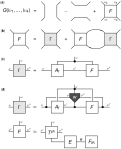
\includegraphics[width=0.8\linewidth]{figure/bse3.pdf}
   \caption{PDFファイルも直接張り込めます。元ファイルはInkscapeで作ったfigure/bse3.svg}
\end{figure}

論文やHPのURLは、\begin{verbatim}\url \end{verbatim}コマンドを使う。

Google, \url{https://www.google.co.jp/}

大関真之. 「今日からできるスパースモデリング」\cite{sparse}。参考文献のbibtexにURLと閲覧日を記入する。

\section{手法}
\clearpage

\section{結果}
\clearpage

\section{まとめと今後の展望}
\clearpage

\section*{謝辞}
本修士論文を執筆する上で多くの方々に助言、協力をいただきました。特に$\cdots$

\bibliography{ref}
\bibliographystyle{junsrt}


\appendix
\section{手法の詳細}
